\documentclass[journal]{IEEEtran}

\usepackage{cite}
\usepackage{graphicx}
\usepackage{array}

\newcommand{\blurb}[1]{\marginpar{{\tt !!!}}{\tt [... #1 ...]}}

\begin{document}

\title{Capture of Individualized Viewers' Interactions in Interactive TV Environments}
\author{Ricardo~Erikson~V.~de~S.~Rosa~and~ 
	Vicente~Ferreira~de~Lucena~Jr.,\IEEEmembership{Member,IEEE,}
	%
\thanks{Ricardo Erikson V. de S. Rosa is with the Graduate Program in Electrical Engineering, Federal University of Minas Gerais, Av. Antônio Carlos 6627, 31270-901, Belo Horizonte, MG, Brazil(e-mail: ricardoerikson@ufmg.br)}%
\thanks{Vicente Ferreira de Lucena Jr. is with the PPGEE, PPGI, and CETELI - Electronics and Information Technology R\&D Center at UFAM, Manaus, Amazonas, Brazil (e-mail: vicente@ufam.edu.br)}%
}

\maketitle

\begin{abstract}
Advances in TV technology have enabled viewers to actively interact with the TV through interactive applications instead of just passively watching TV. Typically, the interactions occur by using a conventional remote control, which is shared by many viewers and hinders the capture of viewers' individual interactions. It is also difficult to identify the context in which the interactions occur, e.g., to manage precisely who is present in the environment and what is being watched on TV. In this paper, it is presented a novel architecture that facilitates the capture of viewers' individual interactions and contextual data in shared TV environments. This architecture uses personal devices as second screen devices with the aim of identifying viewers and capturing their interactions with interactive TV devices.
\end{abstract}

\begin{IEEEkeywords}
Interactive TV; Second Screen; Web Applications
\end{IEEEkeywords}

\IEEEpeerreviewmaketitle

\section{Introduction}

TV watching is essentially a social activity, where groups of people with a common interest share the same space and TV set for entertainment or information. After many advances in technologies for interactive TV (iTV), it is possible to develop high-level applications to enrich the watching experience. Thus, the interaction between viewers and TV became more elaborated than simply change channels and adjust sound volume. Many iTV products, such as Google TV, Apple TV and smart TVs from several manufactures have contributed significantly to this scenario, since they carry a wide variety of services, e.g., news, games and shopping.

The data that is collected from viewers during their interactions with iTV services can provide valuable information for iTV personalization, specially when it is individualized and comes from millions of viewers~\cite{Teixeira2010}. Unfortunately, the traditional model of interaction between viewer and TV, which uses a conventional remote control (RC), hinders to obtain this individualized data~\cite{Cesar2008}. The only existing remote control is shared by many viewers and it is difficult to manage who is in possession of the remote control at a given moment. Consequently, it is also difficult to provide high quality personalization, since the tastes that were inferred from the users in charge of the RC can be imposed on the tastes of the others.

In this paper it is presented a novel secondary screen architecture to capture individualized viewers' interactions with iTV services. Personal devices (e.g., smartphones and tablets) are used as secondary screens with the aim of capturing personal interactions from each viewer that is actively interacting with the iTV terminal.In addition, the interactive capabilities of personal devices can provide a powerful interface for users~\cite{Lee2013}.

\section{Overview of the Second Screen Architecture}

The overall architecture of the system is presented in \figurename~\ref{fig_architecture}. This architecture consists of tree parts that interact with each other: (1) second screen devices, which are the personal devices; an (2) iTV terminal; and (3) the web application. The web application is hosted in the content provider (CP) infrastructure, which comprises the computing resources (e.g., application server, database services and storage services) that are necessary to host web applications.

% Trocar essa figura
\begin{figure}[!t]
	\centering
	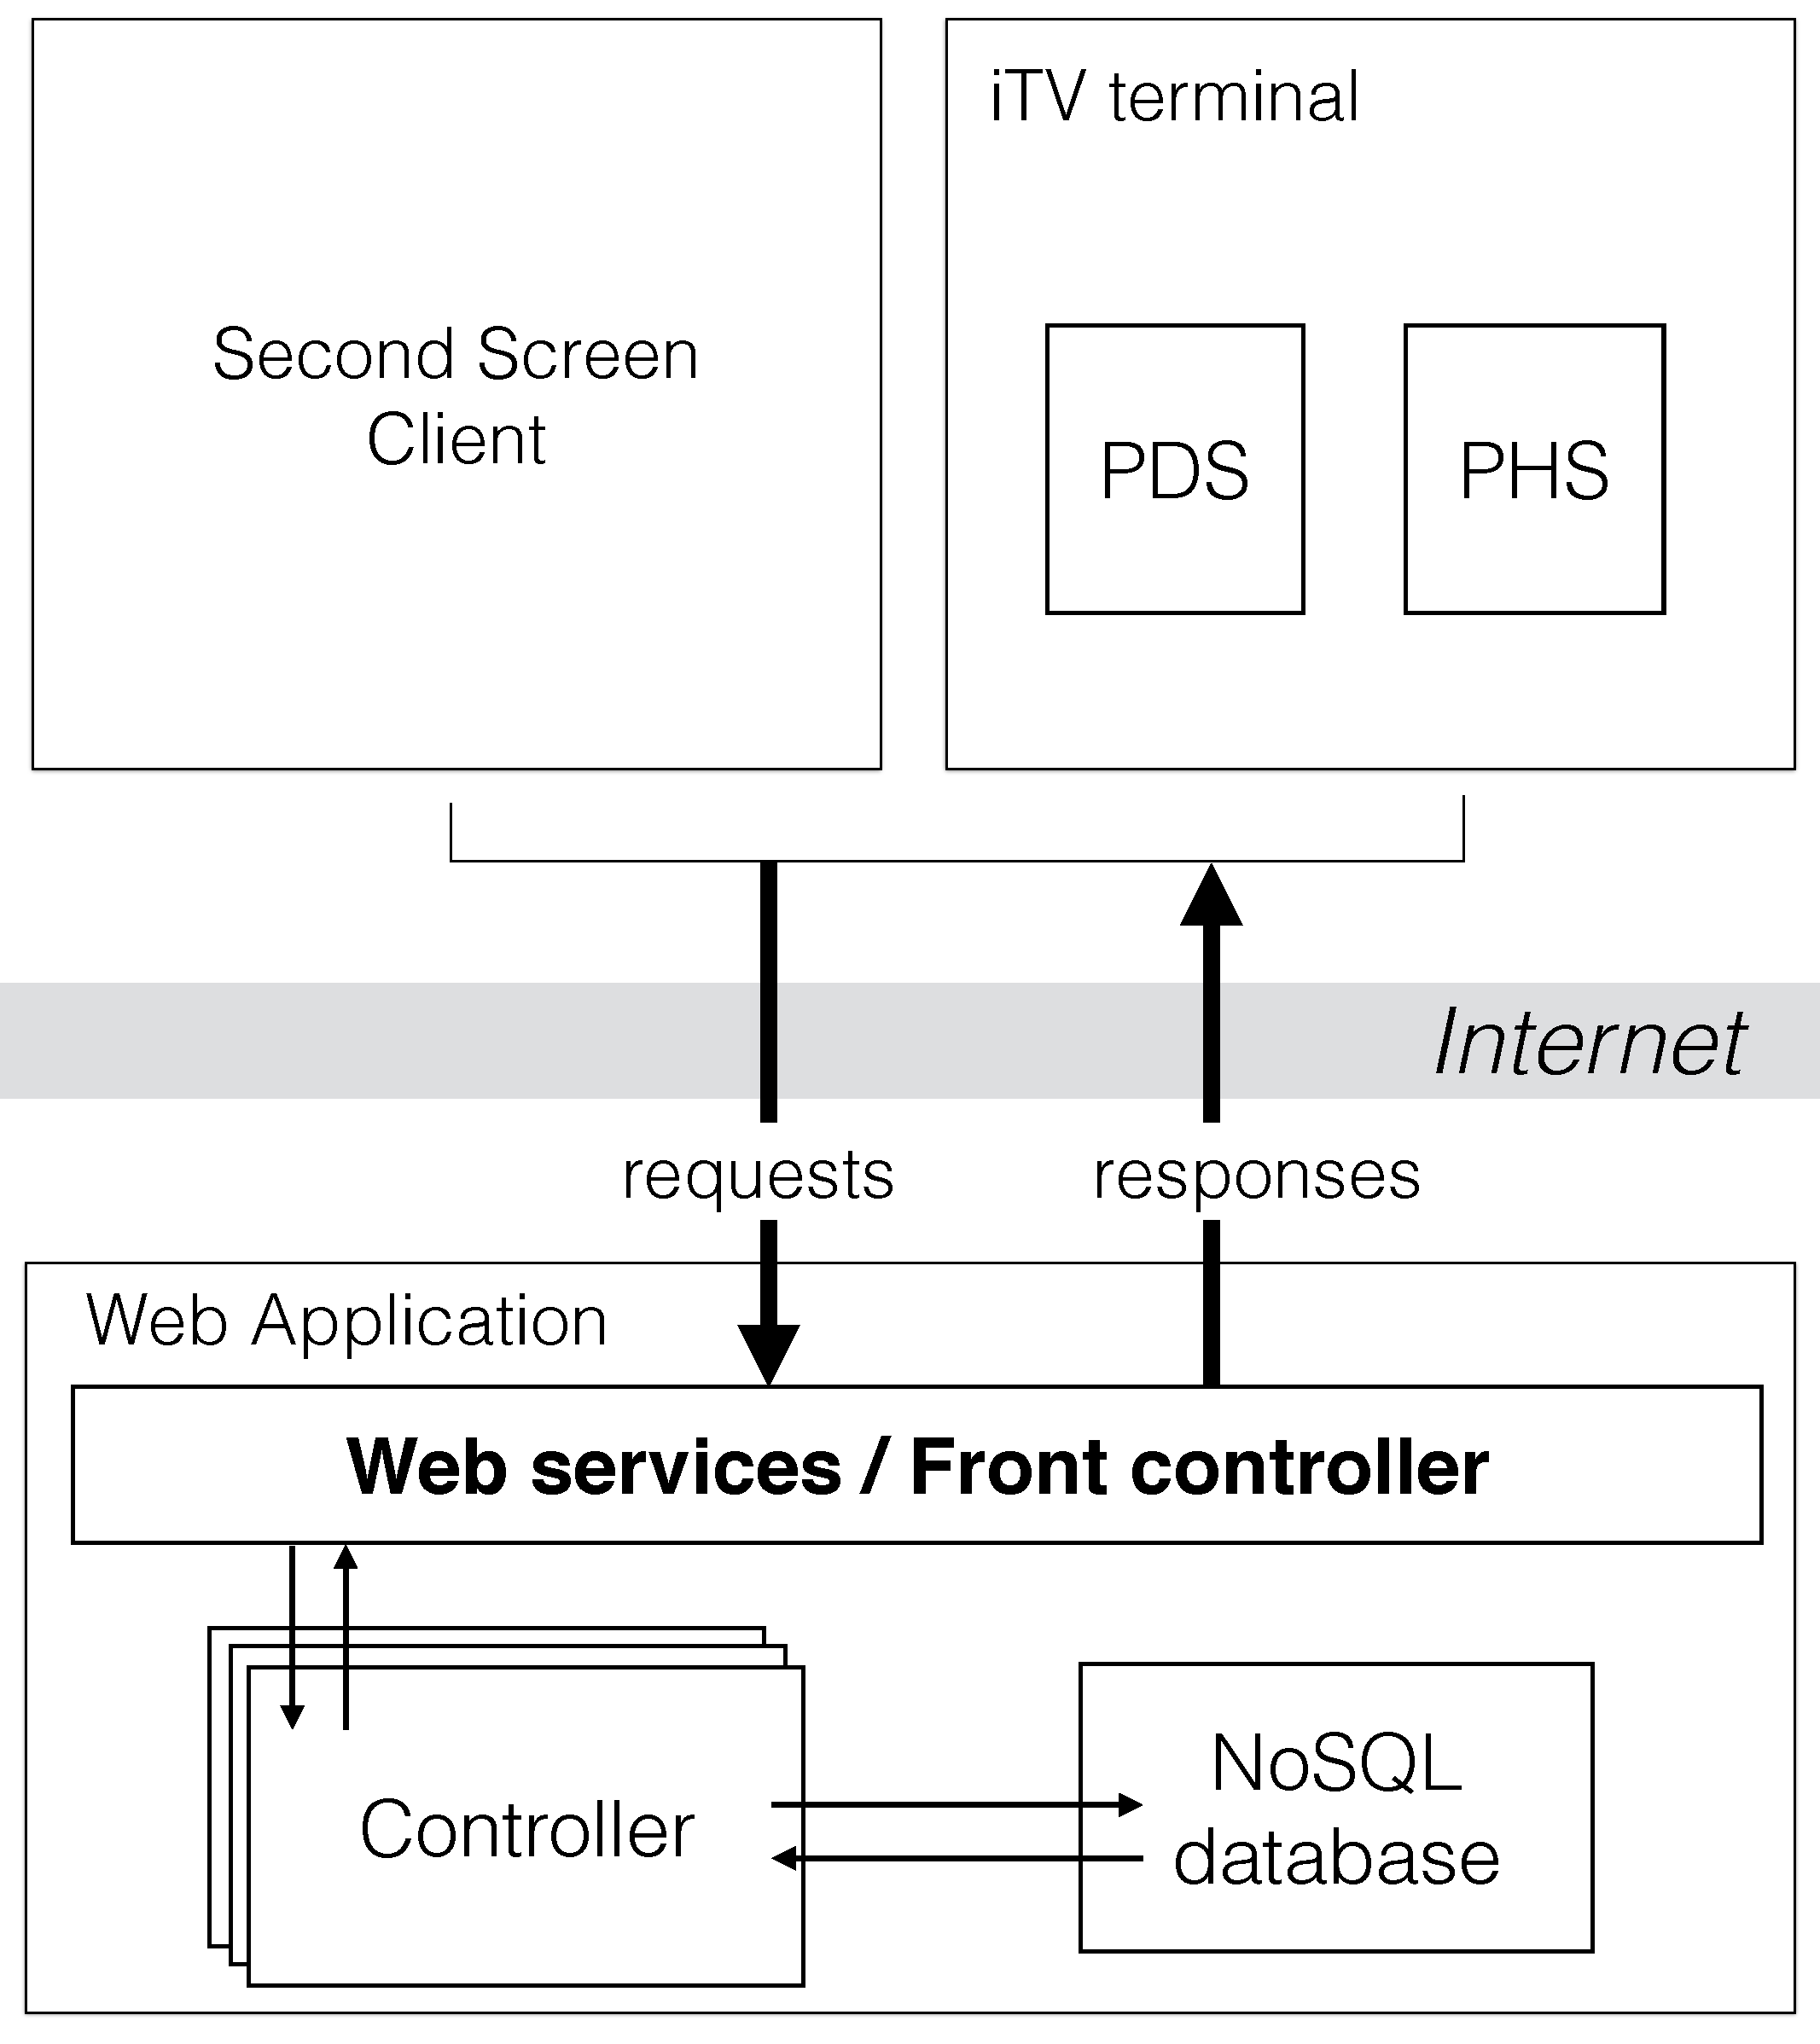
\includegraphics[width=3.5in]{img/architecture-overview.pdf}
	\caption{Architecture to capture viewers' interactions. The data is captured and stored in the CP infrastructure.}
	\label{fig_architecture}
\end{figure}

The web application contains web services that are designed for interoperability between the second screen devices, the iTV terminal and the CP infrastructure. This web application contains business logic for storing and processing the interaction data obtained from the viewers. By using the web services, second screen clients can perform requests to the web application with the purpose of obtaining resources and sending data. 

In the web application, an authentication mechanism must be provided so that the viewers can connect their second screen devices and iTV terminals (e.g., set-top boxes or smart TVs) with an user account. Once the authentication is completed, the second screen device can be used to interact with the iTV terminal. By using the authentication mechanism and considering the second screen client as being a personal device, every user interacting with the iTV terminal can be properly identified.

Once the second screen devices are authenticated, a Presence Detector Service (PDS) in the iTV terminal detects physically nearby devices that have the services that are necessary to establish a communication with an iTV terminal. A Profile Handler Service (PHS) performs profile management when new second screen devices are found in the iTV environment. Thus, only authorized devices can communicate with the iTV terminals. This feature is particularly appropriate for the TV environment, since the second screen devices are usually connected with an iTV terminal via a short range wireless communication technology, e.g., WiFi or Bluetooth.

\section{Implementation of the iTV Environment using Second Screen}

The architecture described in this paper combines several concepts and technologies, e.g. second screen, interactive television, mobile applications, device to device communication and web technologies. An implementation of this architecture was developed using the Java programming language in both server and client. However, the proposed approach does not require uniquely the Java programming language and its use does not subtract the generality of the architecture. Indeed, the architecture can be implemented in other languages provided that they are compatible with the development platforms.

A open source web framework~\cite{Walls2011} was used to develop the server side of the architecture, i.e., the web application. This framework facilitates the development of the front controller pattern in web-based applications. Thus, all the requests are tunneled through a single entry point, which is an efficient way to implement a command-based mechanism. This mechanism not only routes and dispatches commands to appropriate handlers, but also exposes a flexible and scalable API structure.

Table~\ref{tab_web_services_design} describes the design of the Unified Resource Identifiers (URIs) to provide a mechanism of interaction between second screen devices and the web application. The CRUD operations can be requested by requested by the second screen client by using a proper resource and selecting a proper HTTP method. The HTTP methods that were used for CRUD were the following: POST, used when it is necessary to create a new resource; GET, used when it is needed a response with the resource specified in the request; PUT, employed to update a resource; and DELETE, used to delete a resource.

\begin{table}[!t]
	\label{tab_web_services_design}
	\renewcommand{\arraystretch}{1.3}
	\caption{Description of the strategies to handle CRUD by combining HTTP methods and URIs.}
	\centering
	\begin{tabular}{|l|c|p{3.5cm}|}
		\hline
		\bfseries Resource & \bfseries HTTP Method & \bfseries Description of the operation
		\tabularnewline\hline
		/resource & GET& Retrieves a list of the specified resource 
		\tabularnewline\hline
		/resource/\emph{\{id\}} & GET & Retrieves a specific resource identified by \emph{\{id\}}
		\tabularnewline\hline
		/resource & POST & Creates a new resource 
		\tabularnewline
		\hline
		/resource/\emph{\{id\}} & PUT & Updates a resource identified by \{id\}
		\tabularnewline
		\hline
		/resource/\emph{\{id\}} & DELETE & Deletes a resource identified by \emph{\{id\}}
		\tabularnewline
		\hline
	\end{tabular}
\end{table}

The second screen clients can retrieve the content from the server in order to present personalized content to the client. This content can be obtained by using a GET request to the specified resource. Second screen clients can also perform requests to send content to the web-application. A special use of this type of request is to track viewers' interactions. Every interaction can be sent to the web application for further processing in order to provide content customization.

An important feature of this implementation is the possibility of deployment under a cloud-computing environment to support requests from millions of iTV viewers~\cite{Lee2010}. In a cloud-computing environment, the data obtained from viewers can be stored in NoSQL databases, which can provide flexibility and scalability in the second screen implementation.

The communication between second screen devices and iTV terminals can be accomplished by using some communication protocol. Usual communication protocols in this type communication include the Anymote protocol, which provides commands for communication between Android devices and iTV terminal, and the push notification mechanism, which enables the communication by means of an intermediary server on the Internet.

\section{Conclusions}

An implementation of a second screen architecture is described in this paper. It was developed in a commercial cloud computing platform, in which the web application is deployed. An experimental application that consists of a content rating system was developed to store  viewers' interactions. This application tracks the viewers' behaviors during their interactions and stores their ratings towards audio visual content. Some web services were developed to provide interoperability among the secondary screen devices and the web application. Thus, the interactions that are captured during the use of the secondary screen application are sent to the web application by means of HTTP requests to the web services.

\bibliographystyle{IEEEtran}
\bibliography{biblio}

\end{document}